% Source: TeX Live TikZ chains library placement semantics.
\documentclass[border=4pt]{standalone}
\usepackage{tikz}
\usetikzlibrary{chains,positioning,arrows.meta}

\begin{document}
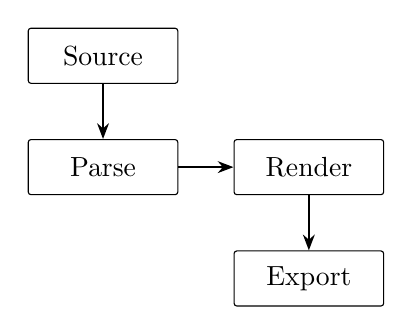
\begin{tikzpicture}[
  node distance=7mm,
  start chain=flow placed below,
  item/.style={draw, rounded corners=1pt, minimum width=19mm, minimum height=7mm, align=center},
  edge/.style={-{Stealth[length=2mm]}, thick}
]
  \node[item,on chain={flow placed {at={(0,0)}}}] (source) {Source};
  \node[item,on chain] (parse) {Parse};
  \node[item,on chain=flow placed right] (render) {Render};
  \node[item,on chain] (export) {Export};

  \draw[edge] (source) -- (parse);
  \draw[edge] (parse) -- (render);
  \draw[edge] (render) -- (export);
\end{tikzpicture}
\end{document}
